\newpage
\section{Problem J \ \ Superdog and Spdddddddddd}
{ \limitfont{}
Input file: Standard Input \par
Output file: Standard Output \par
Time limit: 1000ms \par
Memory limit: 512MB \par
}
\subsection*{题目描述}
Superdog和Spdddddddddd最近沉迷扫雷。但是,由于Superdog和Spdddddddddd的手速不相上下,速度上的比拼让他们非常疲惫与无聊。

Superdog突发奇想,想到了一种更加刺激(玄学)的方法进行游戏。他们通过第一次点击后,出现的所有数字的加和来决定胜负。如果为奇数,则Superdog获胜。否则,Spdddddddddd获胜。

本题中,扫雷遵循下面的规则:
\begin{itemize}
    \item 在任意时刻,只要某个格子格子被翻开,如果「周围格子」都没有雷,这个格子的「周围格子」会被立刻翻开。被翻开的「周围格子」会递归地应用此规则。
    \item 对于不同位置的格子,其「周围格子」如下所示
\end{itemize}

\begin{figure}[H]
    \centering
    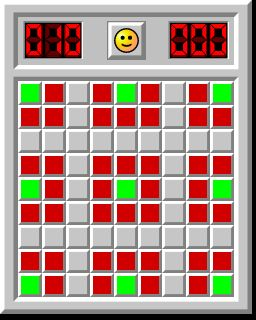
\includegraphics[scale=0.5]{./src/d1.png}
\end{figure}
每个绿色格子周围的红色格子是其「周围格子」

样例2的游戏图:
\begin{figure}[H]
    \centering
    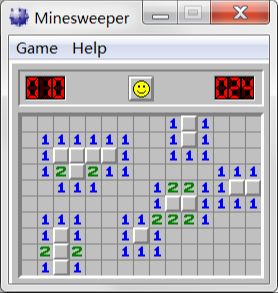
\includegraphics[scale=0.5]{./src/d2.png}
\end{figure}
所有数字累加和为65。
\subsection*{输入描述}
第一行四个整数$m,n,a,b$,代表扫雷格点的长度和宽度,以及第一次点击的格子坐标$(a,b)$。

接下来输入一个$m$行$n$列的$01$矩阵,$0$代表这个点没有雷,$1$代表这个点有雷。

本题中左上角坐标为$(1,1)$,保证第一次不会点到雷。

$1 < n, m \le 500$。
\subsection*{输出描述}

如果Superdog获胜则输出``Superdog''。

如果Spdddddddddd获胜,则输出``Spdddddddddd''。

\subsection*{测试样例}

\begin{table}[H]
\begin{tabularx}{\textwidth}{|X|X|}
    \hline
    \textbf{Standard Input} & \textbf{Standard Output} \\ 
    \hline 
    \tablecell{
        10 9 1 9 \\
        100000000 \\
        000000000 \\
        000000000 \\
        010100001 \\
        000000000 \\
        000000000 \\
        101000000 \\
        001100000 \\
        000010001 \\
        000000100 \\
    } & 
    \tablecell{Spdddddddddd \\ \\ \\ \\ \\ \\ \\ \\ \\ \\ \\} \\
    \hline
    \tablecell{
        10 15 1 1 \\
        000000000000000 \\
        000000000010000 \\
        001001000000000 \\
        000100000000000 \\
        000000000000010 \\
        000000000110000 \\
        000000000000000 \\
        001000010000000 \\
        000000000000000 \\
        001000000000000 \\
    } & \tablecell{
        Superdog \\ \\ \\ \\ \\ \\ \\ \\ \\ \\ \\
    } \\
    \hline
\end{tabularx}
\end{table}

